\documentclass{mc2015}

%%%%%%%%%%%%%%%%%%%%%%%%%%%%%%%%%%%%%%%%%%%%%%%%%%%%%%%%%%%%%%%%%%%%%
\usepackage[T1]{fontenc}         % Use T1 encoding instead of OT1
\usepackage[utf8]{inputenc}      % Use UTF8 input encoding
\usepackage{microtype}           % Improve typography
\usepackage{booktabs}            % Publication quality tables
\usepackage{amsmath}
\usepackage{graphicx}
\usepackage{float}
\usepackage{subcaption}
\usepackage[exponent-product=\cdot]{siunitx}
\usepackage[colorlinks,breaklinks]{hyperref}
\hypersetup{linkcolor=black, citecolor=black, urlcolor=black}

\allowdisplaybreaks

\usepackage{lipsum}

\newcommand{\fig}[1]{Fig.~\ref{#1}}                      % figure
\newcommand{\figs}[2]{Figs.~\ref{#1}-\ref{#2}}     
\newcommand{\tbl}[1]{Table~\ref{#1}}                     % table

\newcommand{\benum}{\begin{equation}} 			% numbered equation
\newcommand{\eenum}{\end{equation}}

\newcommand{\beanum}{\begin{eqnarray}}  % numbered equation array
\newcommand{\eeanum}{\end{eqnarray}}

\newcommand{\eqt}[1]{Eq. (\ref{#1})}  % Reference to one equation
\newcommand{\eqts}[1]{Eqs. (\ref{#1})}  % Reference to multiple equations 

\newcommand{\B}[1]{\ensuremath{{B_{#1} }}}
\newcommand{\J}{\ensuremath{\mathbf{J} }}
\newcommand{\p}{\ensuremath{ \partial}}
\newcommand{\M}{\ensuremath{ \mathbf M}}
\newcommand{\Mw}{\ensuremath{\widehat{\mathbf M}}}

\newcommand{\abs}[1]{\ensuremath{\left\lvert #1 \right\rvert}}
\newcommand{\norm}[1]{\ensuremath{\left\lVert #1 \right\rVert}}

\newcommand{\BCSZ}{\ensuremath{\widetilde{\psi}_{BCSZ}}}
\newcommand{\BCSZH}{\ensuremath{\widehat{\psi}_{BCSZ}}}

\newcommand{\omg}{\ensuremath{\vec{\Omega}}}

\newcommand{\pec}{\, ,}
\newcommand{\pep}{\, .}

\def\equationautorefname{Eq.}
\def\figureautorefname{Fig.}

%%%%%%%%%%%%%%%%%%%%%%%%%%%%%%%%%%%%%%%%%%%%%%%%%%%%%%%%%%%%%%%%%%%%%
% Insert authors' names and short version of title in lines below

\authorHead{Maginot, Ragusa, and Morel}
\shortTitle{BCSZ}

%%%%%%%%%%%%%%%%%%%%%%%%%%%%%%%%%%%%%%%%%%%%%%%%%%%%%%%%%%%%%%%%%%%%%
\begin{document}

\title{A Non-negative, Non-linear, Petrov-Galerkin Method for Bilinear Discontinuous differencing of the $S_N$ Equations}

\author{Peter G. Maginot}
\author{Jean C. Ragusa\footnote{Corresponding author} }
\author{Jim E. Morel}
\affil{Department of Nuclear Engineering\\
Texas A\&M University \\
  3133 TAMU, College Station, TX 77843 \\
 pmaginot@tamu.edu; jean.ragusa@tamu.edu; morel@tamu.edu}

\maketitle

\begin{abstract}
We have developed a new, non-negative, non-linear, Petrov-Galerkin bilinear discontinuous  
(BLD) finite element differencing of the 2-D Cartesian geometry $S_N$ equations for quadrilaterals on an unstructured mesh.  
This work is an extension of a scheme we previously developed for use with linear discontinuous (LD) differencing of the 2-D $S_N$ equations for rectangular mesh cells.
We present the theory and equations that describe the new method.  
Additionally, we numerically compare the accuracy of our proposed method to the accuracy of BLD without lumping and the subcell corner balance method (equivalent to a ``fully'' lumped BLD scheme) for a test problem that causes BLD scheme to generate negative angular flux solutions.

\emph{Key Words}: Radiation transport, DFEM, non-negative, bilinear, quadrilaterals
\end{abstract}

%% Final PDF file size should be no more than 4 MB.  Recommended paper length is 10-12 pages.  %%

%%%%%%%%%%%%%%%%%%%%%%%%%%%%%%%%%%%%%%%%%%%%%%%%%%%%%%%%%%%%%%%%%%%%%
\section{Introduction}

%
% - Negativities are a problem in DFEM radtran
% - Need bilinear dfem for thick diffusion limit (cite Adams paper)
% - Solution method like CSZ paper, not Don's paper
%
%

Discontinuous finite element method (DFEM) spatial discretizations of the $S_N$ neutron transport equation and $S_N$ thermal radiative transfer equations can result in negative angular flux and negative angular intensity solutions.  
These negative solutions are non-physical, but inherent to the mathematics that define the radiation spatial differencing scheme.
Several researchers have examined different methods (matrix lumping\cite{adams_dfem}, fix-ups\cite{fichtl}, and strictly non-negative solution representations\cite{csz_me}) that inhibit or eliminate the negativities of the linear discontinuous (LD) finite element scheme on  a variety of spatial mesh cell types for the $S_N$ neutron transport equation.
However, Adams showed that LD does not maintain the neutronics thick diffusion limit on quadrilaterals \cite{adams_dfem}.
We are interested in accurate methods for radiative transfer, therefore we seek methods that can maintain the equilibrium diffusion limit on quadrilaterals.
If a radiative transfer spatial discretization is to maintain the equilibrium diffusion limit, its neutron transport analog must preserve the thick diffusion limit.
As a first step towards accurate methods for radiative transfer on quadrilaterals, we seek a new, non-negative, finite element discretization that the maintains the bilinear spatial moments of the neutron transport equation on quadrilaterals.

The unlumped bilinear discontinuous (UBLD) spatial scheme yields negative angular flux solutions for quadrilateral cells with grazong radiation incidence and/or large optical thickness \cite{adams_dfem}. 
To our knowledge, only matrix lumping has been considered  in an attempt to inhibit negative angular flux solutions of BLD spatial discretizations.
While more common forms of matrix lumping, such as mass matrix or combination mass and surface matrix lumping, inhibit negative angular flux solutions, they do not guarantee a strictly non-negative BLD angular flux solution  for source-free pure absorber problems\cite{adams_dfem}.
Wareing, et al., derived the fully lumped BLD (FLBLD) scheme \cite{flbld} that uses additional manipulations of the UBLD equations to yield angular flux solutions that are strictly non-negative for source-free pure absorber problems.
Unfortunately, Adams demonstrated that FLBLD, which is equivalent to the subcell balance method on rectangles, is less accurate than unlumped BLD (UBLD) scheme for spatial mesh cells of thin and intermediate thicknesses \cite{adams_scb}.

In \cite{csz_me}, we developed a non-negative, non-linear Petrov-Galerkin DFEM spatial differencing scheme that maintains the linear discontinuous spatial moments of the $S_N$ neutron transport equations in slab and rectangular Cartesian geometry.  
In this paper, will extend the main idea of \cite{csz_me} to create a non-negative, non-linear Petrov-Galerkin DFEM scheme that will maintain the bilinear discontinuous spatial moments of the neutron transport equation on quadrilaterals.
The remainder of this paper is divided as follows: a brief derivation common to all bilinear DFEM is given in Section \ref{sec:mom_eqs}, description and derivation of our new, bilinear consistent set-to-zero (BCSZ) Petrov-Galerkin DFEM scheme is given in Section \ref{sec:bcsz},  computational results demonstrating the strictly positive nature of BCSZ and its improved accuracy relative to UBLD and FLBLD are given in Section \ref{sec:results}, and conclusions are given in Section \ref{sec:conclusions}.

\section{Moment Equations}
\label{sec:mom_eqs}
We begin by first considering the 2-D Cartesian discrete ordinates transport equation:
\benum
\omg_d \cdot \nabla \psi_d(x,y) + \sigma_t(x,y) \psi_d(x,y) = S_d(x,y) \pec
\label{eq:exact_transport}
\eenum
where $\omg_d$ is the neutron direction, $\psi_d(x,y)$ is the angular flux $[n/(cm^s ~sec ~ ster)]$ in direction $\omg_d$, $\sigma_t(x,y)$ is the total interaction cross section $[cm^{-1}]$, and $S_d(x,y)$ is the total source (scattering + fixed sources) in direction $\omg_d$.
Following the standard Galerkin procedure, we take the spatial moment of \eqt{eq:exact_transport} with respect to basis function $\B{i}(x,y)$  by first multiplying by basis function $\B{i}(x,y)$  and integrating over spatial cell $K$.
Assuming cell-wise constant $\sigma_t$, the $i-\text{th}$ spatial moment is:
\benum
\label{eq:mom_ex}
\int_{K}{\B{i}(x,y) \left[\omg_d \cdot \nabla \psi_d(x,y) + \sigma_t \psi_d(x,y) \right]~dx dy} = \int_K{ \B{i}(x,y)S(x,y)~dxdy} \pep
\eenum 
Using integration by parts \eqt{eq:mom_ex} becomes:
\begin{multline}
(\omg_d \cdot \vec{n})\oint_K{ \B{i}(x,y) \psi_d(x,y)~d\ell} - \int_{K}{\psi_d(x,y)\left[\omg_d\cdot\left(\nabla_{xy} \B{i}(x,y)\right)  \right]dxdy} \\ 
+ \sigma_t\int_K{ \B{i}(x,y) \psi_d(x,y)~dxdy} \pep
\end{multline}
Defining a reference element mapping as in \fig{fig:ref_map}:
\begin{figure}[t]
\centering
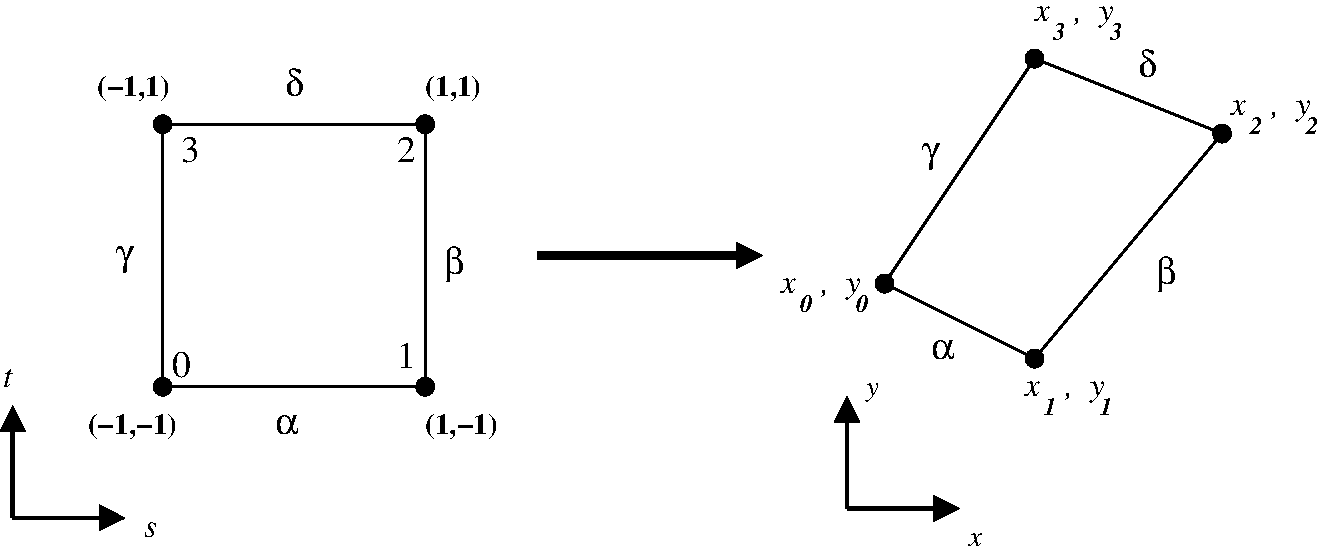
\includegraphics[width=4.5in]{mc_coord.pdf}
\caption{Reference element mapping.}
\label{fig:ref_map}
\end{figure}
a reference point $(s,t)$, $s\in[-1,1]~t\in[-1,1]$, is transformed to a physical point $(x,y)$ such that:
\beanum
x &=& x_0 \B{0}(s,t) + x_1 \B{1}(s,t) + x_2 \B{2}(s,t) + x_3 \B{3}(s,t) \\
y &=&  y_0 \B{0}(s,t) + y_1 \B{1}(s,t) + y_2 \B{2}(s,t) + y_3 \B{3}(s,t) \pep
\eeanum
In this work, we use mapped, bilinear Lagrange interpolatory functions as basis functions:
\begin{subequations}
\label{eq:basis_func}
\beanum
\B{0}(s,t) &=& \frac{1-s}{2}\frac{1-t}{2} \\
\B{1}(s,t) &=& \frac{s+1}{2}\frac{1-t}{2} \\
\B{2}(s,t) &=& \frac{s+1}{2}\frac{t+1}{2} \\
\B{3}(s,t) &=& \frac{1-s}{2}\frac{t+1}{2}  \pep
\eeanum
\end{subequations}
With this choice of basis functions, following the Galerkin procedure creates four equations with more unknowns than equations.
To solve the moment equations, one must assume a solution representation, $\widetilde{\psi}_d(s,t)$, to approximate the true angular flux, $\psi_d(s,t)$.

%For every direction $\omg_d$, the four, exact, bilinear moment equations are:
%\begin{small}
%\begin{subequations}
%\label{eq:mom_eqs}
%\beanum
%(\omg \cdot \vec{n}_{\alpha})\psi_{1,\alpha} + 
%(\omg \cdot \vec{n}_{\beta})\psi_{1,\beta} + (\omg \cdot \vec{n}_{\delta})\psi_{1,\delta}+
%(\omg \cdot \vec{n}_{\gamma})\psi_{1,\gamma} - \mu \psi_{1,\mu} - \eta \psi_{1,\eta} + \sigma_t\psi_{1,M} &=& S_{1,M} \\
%%
%%
%(\omg \cdot \vec{n}_{\alpha})\psi_{2,\alpha} + 
%(\omg \cdot \vec{n}_{\beta})\psi_{2,\beta} + (\omg \cdot \vec{n}_{\delta})\psi_{2,\delta}+
%(\omg \cdot \vec{n}_{\gamma})\psi_{2,\gamma} - \mu \psi_{2,\mu} - \eta \psi_{2,\eta} + \sigma_t\psi_{2,M} &=& S_{2,M} \\
%%
%%
%(\omg \cdot \vec{n}_{\alpha})\psi_{3,\alpha} + 
%(\omg \cdot \vec{n}_{\beta})\psi_{3,\beta} + (\omg \cdot \vec{n}_{\delta})\psi_{3,\delta}+
%(\omg \cdot \vec{n}_{\gamma})\psi_{3,\gamma} - \mu \psi_{3,\mu} - \eta \psi_{3,\eta} + \sigma_t\psi_{3,M} &=& S_{3,M} \\
%%
%%
%(\omg \cdot \vec{n}_{\alpha})\psi_{4,\alpha} + 
%(\omg \cdot \vec{n}_{\beta})\psi_{4,\beta} + (\omg \cdot \vec{n}_{\delta})\psi_{4,\delta}+
%(\omg \cdot \vec{n}_{\gamma})\psi_{4,\gamma} - \mu \psi_{4,\mu} - \eta \psi_{4,\eta} + \sigma_t\psi_{4,M} &=& S_{4,M} \pec
%\eeanum
%\end{subequations}
%\end{small}
%where we have defined the following quantities as a function of basis function \B{i}:
%\begin{subequations}
%\label{eq:mom_defs}
%\beanum
%\psi_{i,\alpha} &=& \frac{\abs{J_{\alpha}}}{2}\int_{-1}^{1}{\B{i}(s,-1)\psi(s,-1)~ds}\\
%\psi_{i,\beta} &=& \frac{\abs{J_{\beta}}}{2}\int_{-1}^{1}{\B{i}(1,t)\psi(1,t)~dt}  \\
%\psi_{i,\delta} &=& \frac{\abs{J_{\delta}}}{2}\int_{-1}^{1}{\B{i}(s,1)\psi(s,1)~ds} \\
%\psi_{i,\gamma} &=& \frac{\abs{J_{\gamma}}}{2}\int_{-1}^{1}{\B{i}(-1,t)\psi(-1,t)~dt} \\
%\psi_{i,\mu} &=& \int_{-1}^1{\int_{-1}^1{\psi(s,t)\left(\frac{\p y}{\p t}\frac{\p \B{i}}{\p s} - \frac{\p y}{\p s}\frac{\p \B{i}}{\p t}  \right) dsdt}} \\
%\psi_{i,\eta} &=& \int_{-1}^1{\int_{-1}^1{ \psi(s,t) \left( \frac{\p x}{\p s}\frac{\p \B{i}}{\p t} - \frac{\p x}{\p t}\frac{\p \B{i}}{\p s} \right)dsdt}} \\
%\psi_{i,M} &=& \int_{-1}^1{\int_{-1}^1{ \B{i}(s,t) \psi \abs{\mathbf J}~dsdt}} \\
%S_{i,M} &=&  \int_{-1}^1{\int_{-1}^1{ \B{i}(s,t) S(s,t) \abs{\mathbf J}~dsdt}} \pep
%\eeanum
%\end{subequations}
%In \eqts{eq:mom_defs}, $\mathbf{J}$ is the Jacobian matrix of the transformation:
%\benum
%\mathbf{J} = \left[ \begin{array}{cc} 
%\frac{\p x}{\p s} & \frac{\p y}{\p s} \vspace{0.1in}\\
%\frac{\p x}{\p t} & \frac{\p y}{\p t}
%\end{array}\right] \pec
%\eenum
%$\abs{J_{\alpha,\beta,\delta,\gamma}}$ is the length of physical element side $\alpha,~\beta,~\delta,~\text{or }\gamma$, respectively, and $\omg_d = \langle \mu , \eta \rangle$.
%Additionally, we remind the reader that for a function, $h(x,y)$ the following hold true\cite{dfem_book}.
%\beanum
%\int_K{h(x,y) dx~dy} &=& \int_{-1}^1{\int_{-1}^1{ h(s,t) \abs{J(s,t) } ~ds~dt}} \\
%\mathbf{J} \left[ \begin{array}{c} \frac{\p f}{\p x} \\ \frac{\p f}{\p y} \end{array} \right] &=& \left[ \begin{array}{c} \frac{\p f}{\p s} \\ \frac{\p f}{\p t} \end{array} \right] \\
%\vec{\nabla}_{xy} h(x,y) &=& \mathbf{J}^{-1} \vec{\nabla}_{st} h(s,t) \pep
%\eeanum
%\eqts{eq:mom_eqs} has more unknowns than equations, requiring the assumption of a solution representation, $\widetilde{\psi}(s,t)$ that approximates the true angular flux solution $\psi(s,t)$.

The UBLD scheme assumes a solution trial space equal to the basis space,
\benum
\widetilde{\psi}_{UBLD} = \sum_{i=0}^3{\psi_{i,UBLD} \B{i}(s,t)  } \pep
\eenum
Under this assumption, the spatial moments of the transport equation become a $4\times 4$ linear system of equations.  
Interested readers are directed to \cite{adams_dfem} or one of the many other papers that have derived and used UBLD on rectangles and quadrilaterals for a more complete derivation.

The FLBLD scheme \cite{flbld,adams_dfem}, alternatively derived as the subcell balance method on quadrilaterals \cite{adams_scb} begins with the UBLD equations then lumps (diagonalizes) the UBLD mass and surface matrices.  The FLBLD equations are then further manipulated to result in a scheme that is yields strictly non-negative solutions for source-free pure absorber solutions.  The FLBLD scheme is second order convergent in space, but can be less accurate than UBLD for cells of intermediate and thin optical thicknesses.  Interested readers are directed to \cite{flbld,adams_dfem,adams_scb} for a more detailed derivation.

The BCSZ scheme is defined as being a bilinear function, $\BCSZH(s,t)$, 
\benum
\BCSZH(s,t) = \sum_{i=0}^3{\psi_{i,BCSZ} \B{i}(s,t)} \pec
\eenum
everywhere \BCSZH is positive and zero otherwise:
\benum
\BCSZ(s,t) = \left \{ \begin{array}{ll}
\BCSZH(s,t) & \BCSZH(s,t) > 0 \\
0	& \text{otherwise}
\end{array}
\right. \pep
\label{eq:bcsz}
\eenum
The initial iterate of \BCSZH~ is $\widetilde{\psi}_{UBLD}$.  If $\widetilde{\psi}_{UBLD} \geq 0 $ everywhere within a cell, $\BCSZ = \widetilde{\psi}_{UBLD}$.
Using the definition of \BCSZ~ given in \eqt{eq:bcsz} turns the four spatial moments of the transport equation into four non-linear equations with four fundamental unknowns, $\psi_{i,BCSZ}$ that describe the bilinear function \BCSZH.

\section{BCSZ Scheme}
\label{sec:bcsz}
For brevity, we omit a complete derivation of the four spatial moment equations.  Rather, we choose to focus on defining the important characteristics of the BCSZ scheme, namely how the BCSZ scheme defines the following moments equation terms:
\begin{enumerate}
\item edge leakage, $\psi_{i,edge}$,
\item cell volume gradients, $\psi_{i,\mu}$ and $\psi_{i,\eta}$, and
\item cell volume moments, $\psi_{i,M}$.
\end{enumerate}
The $\psi_{i,edge}$ terms come from the moment equation integration by parts:
\begin{subequations}
\label{eq:psi_alpha}
\begin{multline}
(\omg_d \cdot \vec{n})\oint_K{ \B{i}(x,y) \psi_d(x,y)~d\ell}  = (\omg_d \cdot \vec{n}_{\alpha})\frac{\abs{J_{\alpha}}}{2}\int_{-1}^{1}{\B{i}(s,-1)\psi_d(s,-1)~ds} \\
+ (\omg_d \cdot \vec{n}_{\beta})\frac{\abs{J_{\beta}}}{2}\int_{-1}^{1}{\B{i}(1,t)\psi_d(1,t)~dt} 
 + (\omg_d \cdot \vec{n}_{\delta})\frac{\abs{J_{\delta}}}{2}\int_{-1}^{1}{\B{i}(s,1)\psi_d(s,1)~ds} \\ +(\omg_d \cdot \vec{n}_{\gamma}) \frac{\abs{J_{\gamma}}}{2}\int_{-1}^{1}{\B{i}(-1,t)\psi_d(-1,t)~dt} \pep
\end{multline}
Defining an edge moment of the angular flux, $\psi_{i,edge}$, we have \eqt{eq:edge_moment}
\begin{multline}
\label{eq:edge_moment}
(\omg_d \cdot \vec{n})\oint_K{ \B{i}(x,y) \psi_d(x,y)~d\ell}  =  (\omg_d \cdot \vec{n}_{\alpha})\frac{\abs{J_{\alpha}}}{2}\psi_{i,\alpha}
+ (\omg_d \cdot \vec{n}_{\beta})\frac{\abs{J_{\beta}}}{2}\psi_{i,\beta} 
 + (\omg_d \cdot \vec{n}_{\delta})\frac{\abs{J_{\delta}}}{2}\psi_{i,\delta} +(\omg_d \cdot \vec{n}_{\gamma}) \psi_{i,\gamma} \pec
\end{multline}
\end{subequations}
where $\abs{J_z}$ is the length of side $z$, $\vec{n}_z$ is the outward directed unit normal of side $z$, and we have used edge short hands ($\alpha,~\beta,~\delta,~\gamma$) as in \fig{fig:ref_map}.  
The cell volume gradients,$\psi_{i,\mu}$ and $\psi_{i,\eta}$ come from:
\begin{subequations}
\label{eq:cell_grad}
\begin{multline}
\int_{K}{\psi_d(x,y)\left[\omg_d\cdot\left(\nabla_{xy} \B{i}(x,y)\right)  \right]dxdy} = \mu \int_{-1}^1{\int_{-1}^1{\psi_d(s,t)\left(\frac{\p y}{\p t}\frac{\p \B{i}}{\p s} - \frac{\p y}{\p s}\frac{\p \B{i}}{\p t}  \right) dsdt}}  \\
+ \eta \int_{-1}^1{\int_{-1}^1{ \psi_d(s,t) \left( \frac{\p x}{\p s}\frac{\p \B{i}}{\p t} - \frac{\p x}{\p t}\frac{\p \B{i}}{\p s} \right)dsdt}}
\end{multline}
or in short,
\benum
\int_{K}{\psi_d(x,y)\left[\omg_d\cdot\left(\nabla_{xy} \B{i}(x,y)\right)  \right]dxdy} = \mu \psi_{i,\mu} + \eta \psi_{i,\eta} \pec
\eenum
\end{subequations}
where $\omg_d = \langle \mu ,\eta \rangle$.
%\psi_{i,\gamma} &=& \frac{\abs{J_{\gamma}}}{2}\int_{-1}^{1}{\B{i}(-1,t)\psi(-1,t)~dt} \\
%\psi_{i,\mu} &=& \int_{-1}^1{\int_{-1}^1{\psi(s,t)\left(\frac{\p y}{\p t}\frac{\p \B{i}}{\p s} - \frac{\p y}{\p s}\frac{\p \B{i}}{\p t}  \right) dsdt}} \\
%\psi_{i,\eta} &=& \int_{-1}^1{\int_{-1}^1{ \psi(s,t) \left( \frac{\p x}{\p s}\frac{\p \B{i}}{\p t} - \frac{\p x}{\p t}\frac{\p \B{i}}{\p s} \right)dsdt}} \\
%\psi_{i,M} &=& \int_{-1}^1{\int_{-1}^1{ \B{i}(s,t) \psi \abs{\mathbf J}~dsdt}} \\
The $\psi_{i,M}$ term comes from the reaction term:
\benum
\sigma_t\int_K{ \B{i}(x,y) \psi_d(x,y)~dxdy} = \sigma_t\int_{-1}^1{\int_{-1}^1{ \B{i}(s,t) \psi_d \abs{\mathbf J}~dsdt}} = \sigma_t \psi_{i,M} \pep
\eenum
In \eqt{eq:cell_grad},  all $\frac{\p}{\p s}$ terms are linear functions in $t$, all $\frac{\p}{\p t}$ terms are linear functions in $s$, and $\mathbf{J}$ is the Jacobian matrix of the coordinate transformation:
\benum
\mathbf{J} = \left[ \begin{array}{cc} 
\frac{\p x}{\p s} & \frac{\p y}{\p s} \vspace{0.1in}\\
\frac{\p x}{\p t} & \frac{\p y}{\p t}
\end{array}\right] \pep
\eenum

\subsection{BCSZ Edge Integration}
Along any edge, there are four possible cases.  Assuming that we are looking at edge $\alpha$, but with easy translation to any other edge:
\begin{enumerate}
\item $\BCSZH > 0$ along whole edge,
\item  $\BCSZH < 0$ along whole edge,
\item $\psi_{0,BCSZ} < 0$, $\psi_{1,BCSZ} > 0$, and
\item $\psi_{0,BCSZ} > 0$, $\psi_{1,BCSZ} <0$.
\end{enumerate}
Case one is straightforward and identical to the integration used by the UBLD scheme. 
Case two is by definition, zero along the integral.
Cases three and four are handled by first determining $s_z$, where $\BCSZH(s_z,-1) = 0$:
\benum
s_z = \frac{\psi_{0,BCSZ}+\psi_{1,BCSZ}}{\psi_{0,BCSZ} - \psi_{1,BCSZ} }
\eenum
Then a two point Gauss quadrature is mapped to the interval $[s_z,1]$ for case 3 and $[-1,s_z]$ for case 4, and the integral of $\psi_{i,\alpha}$
is computed (exactly) using function evaluations at the mapped quadrature points.

\subsection{BCSZ Cell Integration}
Given the definition of \BCSZ~ in \eqt{eq:bcsz}, the integral contributions to $\psi_{i,\mu},~\psi_{i,\eta},~\text{and }\psi_{i,M}$ are non-trivial only over a portion of the cell where $\BCSZH(s,t) > 0$.
There are seven possible geometric integration cases to be considered for all values of \BCSZH.  Six are shown in \fig{fig:bcsz_cases}.
\begin{figure}[h]
\begin{center}
	\begin{subfigure}{0.32\textwidth}
		\begin{center}
		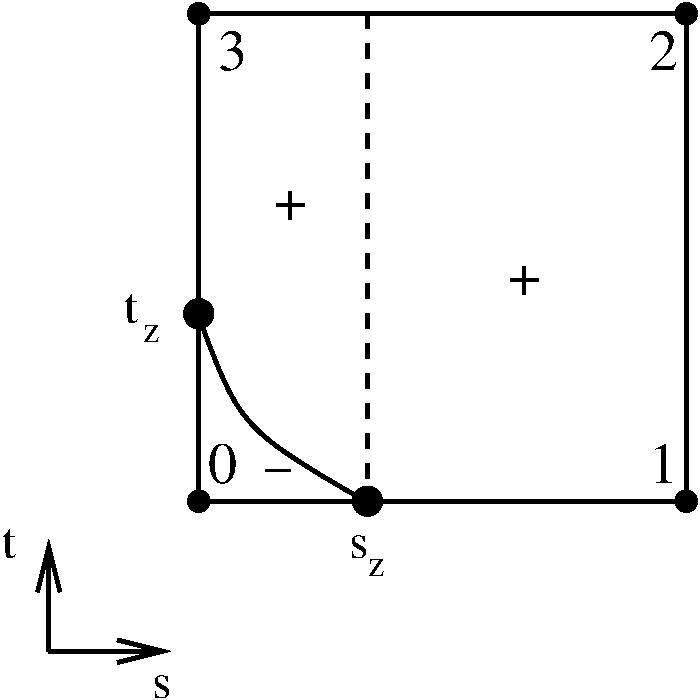
\includegraphics[width=1.75in]{one_neg_pdt_int} 		
		\caption{One negative}
		\label{fig:one_node}
		\end{center}
	\end{subfigure}
	\begin{subfigure}{0.32\textwidth}
		\begin{center}
		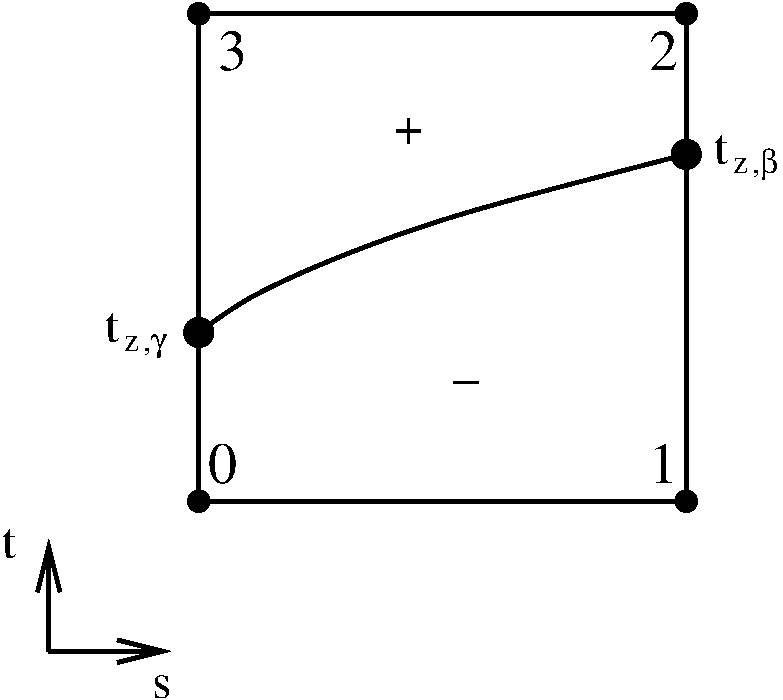
\includegraphics[width=1.75in]{neg_same_side_pdt_int}
		\caption{Two negative, same side}
		\label{fig:two_same_side}
		\end{center}
	\end{subfigure}
	\begin{subfigure}{0.32\textwidth}
		\begin{center}
		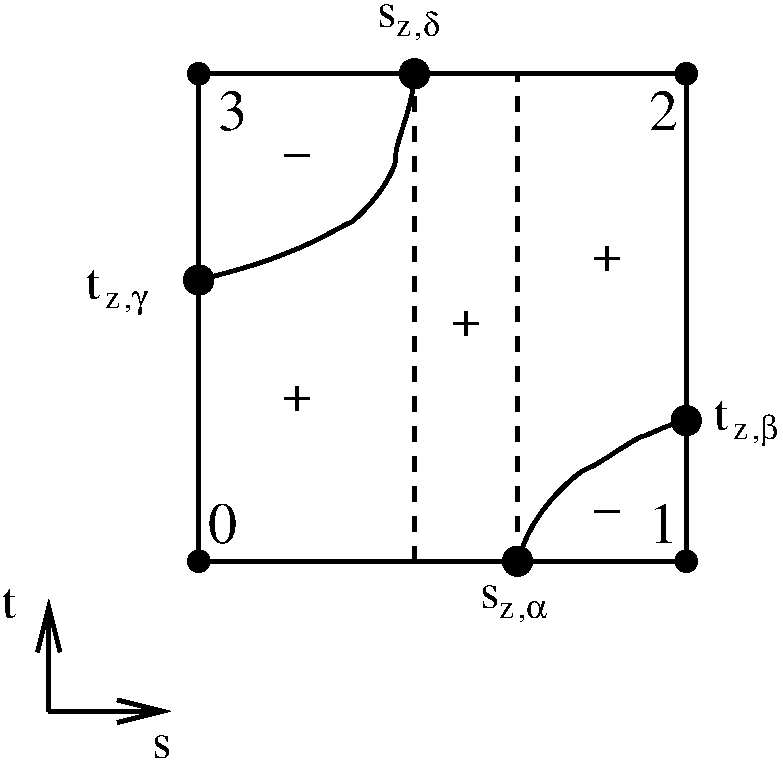
\includegraphics[width=1.75in]{opp_neg_more_pos_pdt_int}
		\caption{Two negative, opposite sides, $\psi_0 \psi_2 > \psi_1 \psi_3$}
		\label{fig:two_opp_more_positive}
		\end{center}
	\end{subfigure}
	\begin{subfigure}{0.32\textwidth}
		\begin{center}
		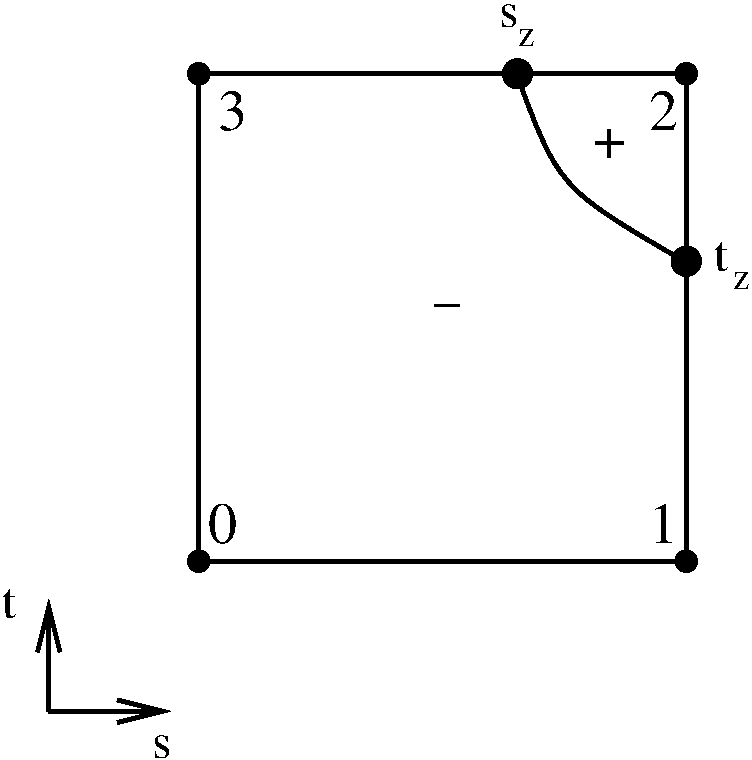
\includegraphics[width=1.75in]{three_neg_pdt_int} 
		\caption{Three negative}
		\label{fig:three_nodes}
		\end{center}
	\end{subfigure}
	\begin{subfigure}{0.32\textwidth}
		\begin{center}
		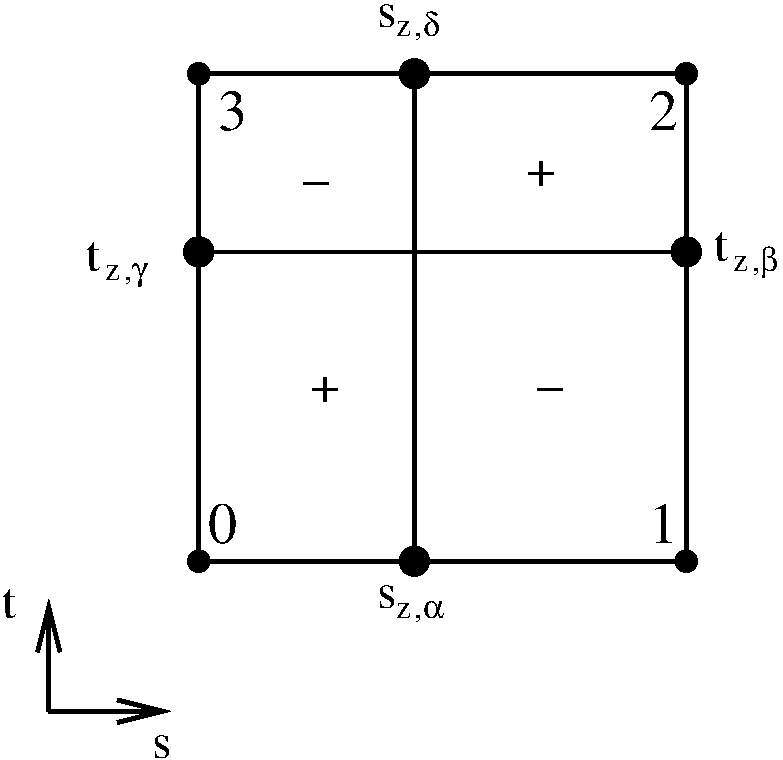
\includegraphics[width=1.75in]{opp_neg_block_pdt_int} 
		\caption{Two negative, block formation, $\psi_1 \psi_3 = \psi_2 \psi_4$}
		\label{fig:two_block}
		\end{center}
	\end{subfigure}
	\begin{subfigure}{0.32\textwidth}
		\begin{center}
		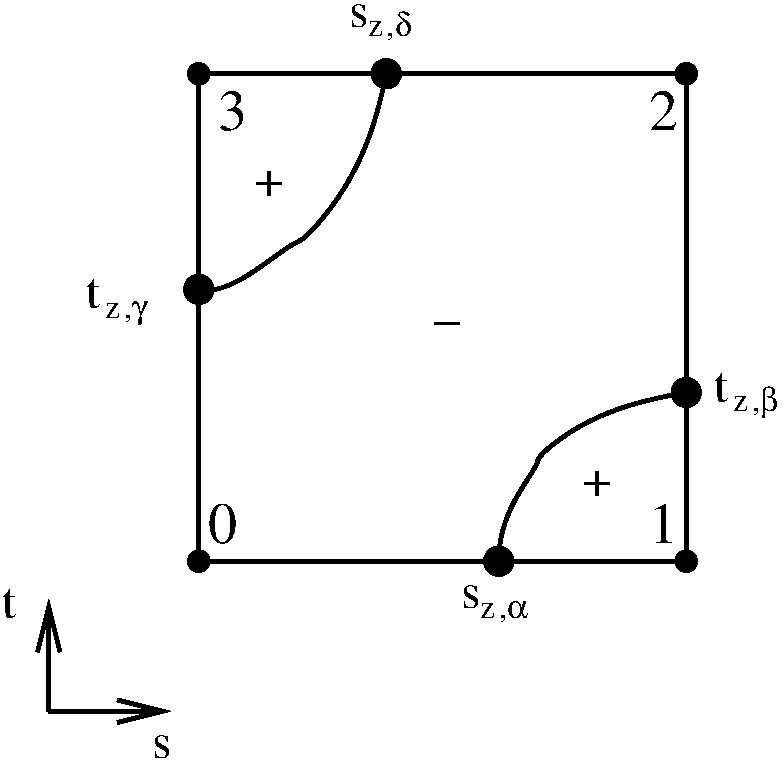
\includegraphics[width=1.75in]{opp_neg_more_neg_pdt_int}
		\caption{Two negative, opposite sides, $\psi_0 \psi_2 > \psi_1 \psi_3$}
		\label{fig:two_opp_negative}
		\end{center}
	\end{subfigure}
	\caption{BCSZ cell integration cases requiring special treatment.}
	\label{fig:bcsz_cases}
	\end{center}
\end{figure}
The other case is when $\BCSZH > 0$ everywhere in the cell, in which case the integration of $\psi_{i,\mu},~\psi_{i,\eta},~\text{and }\psi_{i,M}$ is straight forward, and identical to that required by the definition of the UBLD scheme.
Though other cases are possible, all can be transformed into one of the cases in \fig{fig:bcsz_cases} via rotation.
$\psi_{i,\mu},~\psi_{i,\eta},~\text{and }\psi_{i,M}$ are evaluated by summing the integral contribution in  each region of a particular case given in \fig{fig:bcsz_cases}
To evaluate $\psi_{i,\mu},~\psi_{i,\eta},~\text{and }\psi_{i,M}$ contributions in a region, $R$, bounded by a curved boundary, we make use of variable limits of integration.
Along the curved boundary of $R$, $\BCSZH=0$, this allows us to determine $t$ as a function of $s$ (or $s$ as a function of $t$).  
To find a variable limit of integration with respect to $t$ as a function of $s$, we first transform \BCSZH~ from an interpolatory polynomial to a moment based polynomial, $f(s,t)$:
\benum
f(s,t) = f_c + s f_s + t f_t + st f_{st} \pep
\label{eq:f_def}
\eenum
The coefficients of $f$ are found formula using the interpolatory definition of the basis functions:
\benum
\left[ 
\begin{array}{cccc}
1 &	 -1	& -1 &  1    \\
1 &		1	& -1	&  -1		\\	
1 &	  1	&  1		&  1		\\
1 &		-1	& 1		&  -1		\\
\end{array}
\right]
\left[
\begin{array}{c}
f_c \\
f_s \\
f_t \\
f_{st} 
\end{array}
\right]
=\vec{\psi}_{BCSZ}
\pec
\eenum
with
\benum
\vec{\psi}_{BCSZ} = \left[ \psi_{0,BCSZ},
\psi_{1,BCSZ},
\psi_{2,BCSZ},
\psi_{3,BCSZ} \right]^T
\pep
\eenum
\eqt{eq:f_def} is then manipulated to find a variable limit of integration with respect to $t$, $\hat{l}_t$, that is a function of $s$:
\benum
\hat{l}_t  = -\frac{f_c + f_s s}{f_t + f_{st} s} \pep
\eenum

Rather than evaluating each $\psi_{i,\mu}$, $\psi_{i,\eta}$, and $\psi_{i,M}$ integral, we evaluate a single, generic, bivariate polynomial integrand that is only a function of $s$ and $t$.
%We find this generic integrand by first expanding the specific \BCSZ~ integrand definitions of $\psi_{i,\mu},~\psi_{i,\eta},~\text{and }\psi_{i,M}$  over  $R$.  
%Starting with the integrand of $\psi_{i,\mu}$,
%\begin{subequations}
%\label{eq:m_expand}
%\begin{multline}
%\BCSZH(s,t) \left(\frac{\p y}{\p t}\frac{\p \B{i}}{\p s} - \frac{\p y}{\p s}\frac{\p \B{i}}{\p t}  \right) =  \left[   f_c + s f_s + t f_t + st f_{st} \right] \dots \\
	%\left(  \left[ y_{t,c} + s y_{t,s}\right] \left[ b_{i,s,c} + t b_{i,s,t} \right] - \left[ y_{s,c} + t y_{s,t}\right] \left[ b_{i,t,c} + s b_{i,t,s} \right]\right) \pec
%\end{multline}
%then the $\psi_{i,\eta}$ integrand:
%\begin{multline}
%\BCSZH(s,t)  \left( \frac{\p x}{\p s}\frac{\p \B{i}}{\p t} - \frac{\p x}{\p t}\frac{\p \B{i}}{\p s} \right)  =  \left[   f_c + s f_s + t f_t + st f_{st} \right] \dots \\
%\left( \left[ x_{s,c} + t x_{s,t}\right] \left[ b_{i,t,c} + s b_{i,t,s} \right] -\left[ x_{t,c} + s x_{t,s}\right]\left[ b_{i,s,c} + t b_{i,s,t} \right] \right) \pec
%\end{multline}
%and finally the $\psi_{i,M}$ integrand:
%\benum
%\B{i}(s,t) \BCSZH(s,t) \abs{J(s,t) } = \left[b_{i,c} + s b_{i,s} + t b_{i,t} + st b_{i,st} \right] \left[   f_c + s f_s + t f_t + st f_{st} \right] \left[ g_c + s g_s + t g_t \right] \pep
%\eenum
%\end{subequations}
%In \eqts{eq:m_expand} we have defined the following:
%\begin{subequations}
%\beanum
%\B{i}(s,t) &=& b_{i,c} + s b_{i,s} + t b_{i,t} + st b_{i,st} \\
%\frac{\p \B{i}}{\p s} &=& b_{i,s,c} + t b_{i,s,t}  \\
%\frac{ \p \B{i} }{\p t} &=&  b_{i,t,c} + s b_{i,t,s} \\
%\abs{\mathbf{J}(s,t) } &=& g_c + s g_s + t g_t \\
%\frac{\p x}{\p s} &=& x_{s,c} + t x_{s,t} \\
%\frac{\p x}{\p t} &=& x_{t,c} + s x_{t,s} \\
%\frac{\p y}{\p s} &=& y_{s,c} + t y_{s,t} \\
%\frac{\p y}{\p t} &=& y_{t,c} + s y_{t,s} \pep
%\eeanum
%\end{subequations}
Using \verb+MATLAB+\cite{matlab},  each integrand is further expanded, then terms of equal degree bivariate polynomials,  $s^m t^n$,  with $0 \leq m \leq 3$, $0 \leq n \leq 3$, are collected.
This allows us to calculate the twelve separate integrations of  $\psi_{i,\mu},~\psi_{i,\eta},~\text{and }\psi_{i,M}$, as the multiplication of twelve unique sets of constants, $\mathbf{C}_{i,\mu}$, $\mathbf{C}_{i,\eta}$, and $\mathbf{C}_{i,M}$, multiplied  by the integrations of a single bivariate  integration, over $R$.

\subsubsection{Symbolic integration versus numerical integration}

Initially, \verb+MATLAB+ symbolic algebra generated expressions for the integration of the generic bivariate polynomial over $R$ were used to evaluate $\psi_{i,\mu},~\psi_{i,\eta},~\text{and }\psi_{i,M}$.  This worked well at low cell counts, but caused the \BCSZ~ non-linear iteration to fail at higher cell counts.
To verify the \verb+MATLAB+ generated expressions, we compared the ``exact'' symbolic algebra generated results for calculating $\psi_{i,M}$ for $\vec{\psi}_{BCSZ} = [-2 ~0.1~200~10]^T$ to the value obtained using $N_s$ Gauss quadrature points in $s$ along the curved boundary.  
A two-point Gauss quadrature in $t$ was used for each corresponding Gauss point in $s$ (tensor product quadrature).  An example of the quadrature layout for $N_s=4$ is given in \fig{fig:quad}.
\begin{figure}[h]
\centering
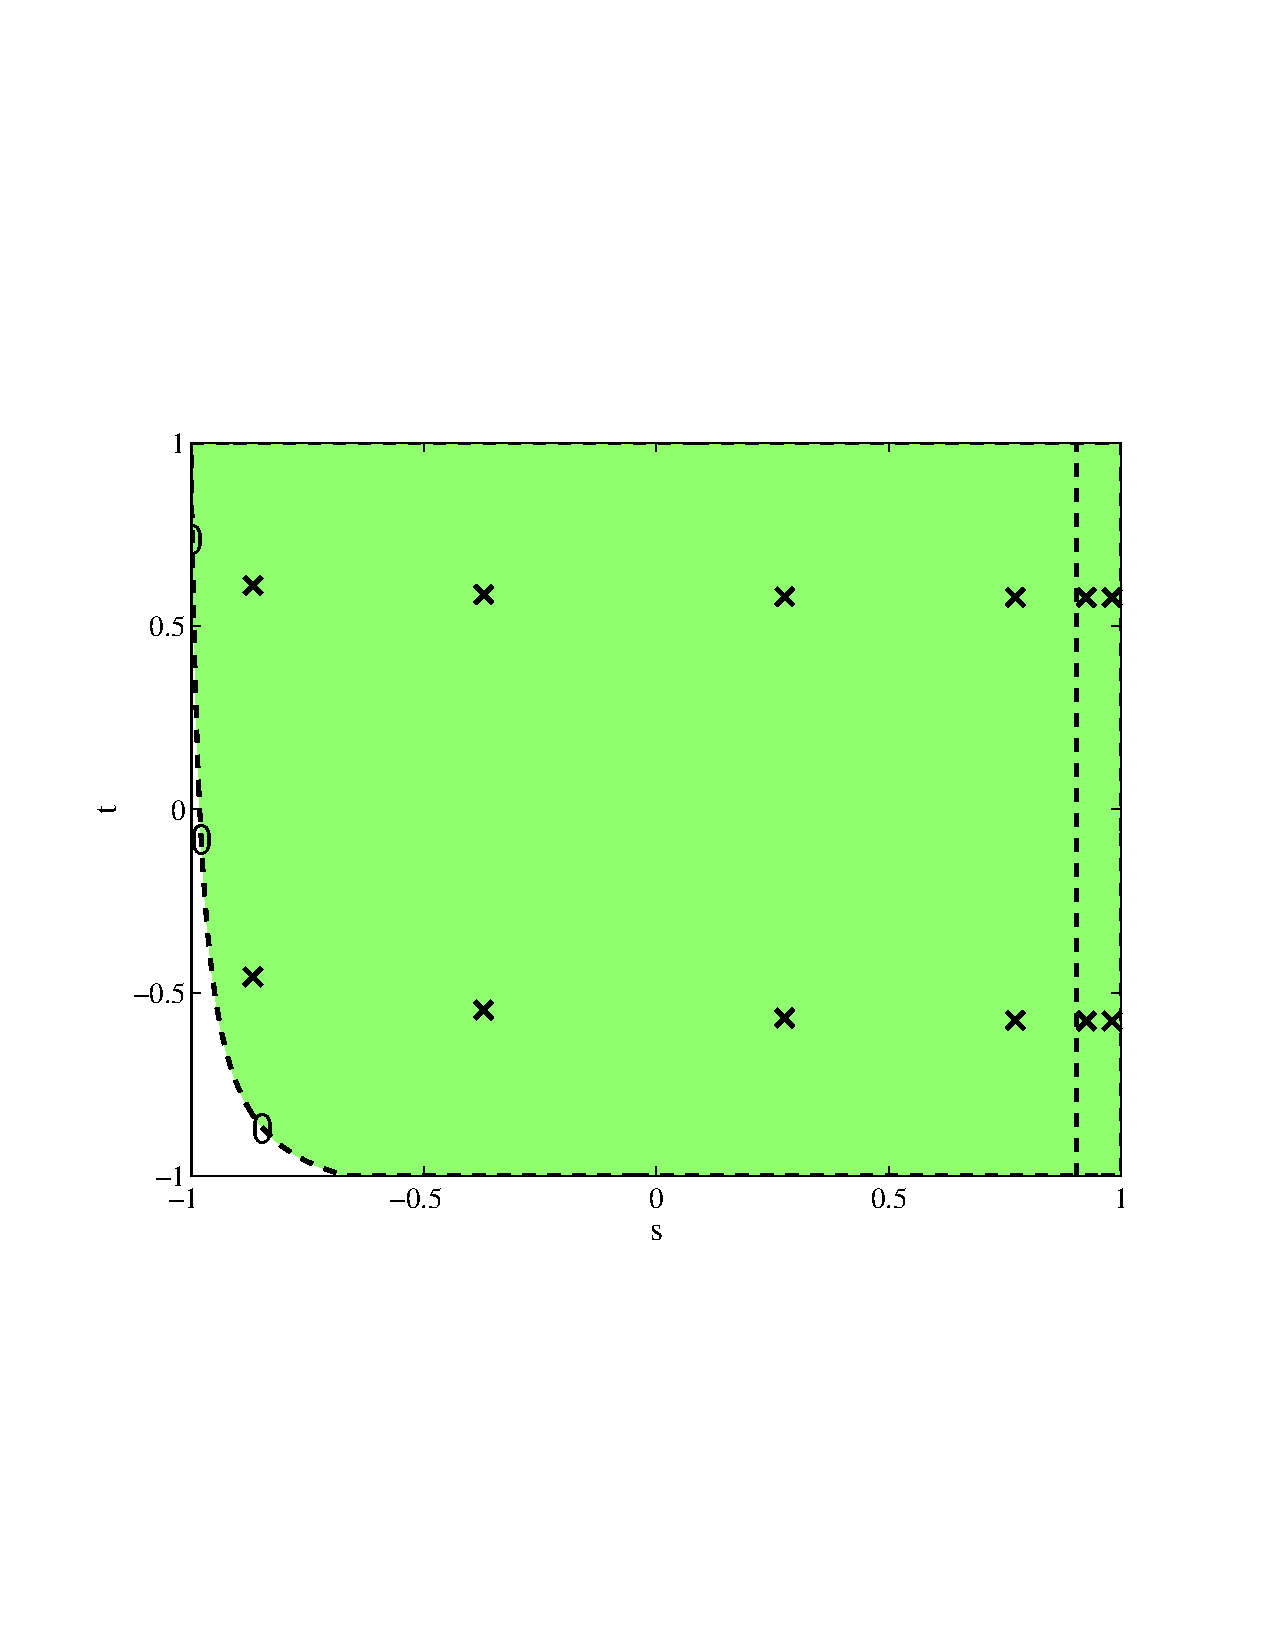
\includegraphics[width=3in,trim=0.5in  2.5in  1.in 2.5in,clip=true]{quad_layout.pdf}
\caption{Quadrature point locations for quadrature integration test.}
\label{fig:quad}
\end{figure}
In \fig{fig:quad_err}, we plot $E_{i,quad}$, where:
\benum
E_{i} = \frac{\abs{ \psi_{i,sym} - \psi_{i,num} }}{\abs{\psi_{i,sym} }} \pec
\eenum
$\psi_{i,sym}$ is the evaluation of $\psi_{i,M}$ using the symbolic algebra generated expressions, and $\psi_{i,num}$ is the quadrature evaluation of $\psi_{i,M}$ using $2N_s + 4$ quadrature points.
Compare the result of \fig{fig:quad_err} to \fig{fig:no_err}, which plots $\widehat{E}_i$:  
\benum
\widehat{E}_{i} = \frac{\abs{ \psi_{i,MAX} - \psi_{i,num} }}{\abs{\psi_{i,MAX} }} \pec
\eenum
where $\psi_{i,MAX}$ is the quadrature approximation of $\psi_{i,M}$ using Gauss quadrature and $N_S = 40$.
Since increasing the number of Gauss quadrature points increases the accuracy of a given quadrature integration, from \fig{fig:error_comparisons} it is clear that the ``exact'' symbolic evaluated expressions suffer from numerical round-off caused by taking the small difference of large numbers.
%
\begin{figure}[h]
\begin{center}
	\begin{subfigure}{0.45\textwidth}
		%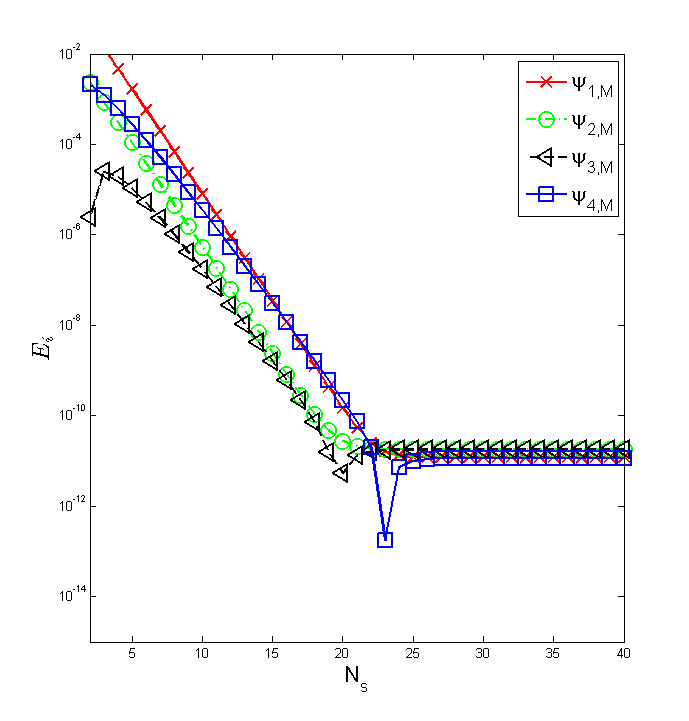
\includegraphics[width=2.5in,trim=0.5in  2.5in  1.0in 2.5in,clip=true]{err_gauss_to_matlab_exact.png}
		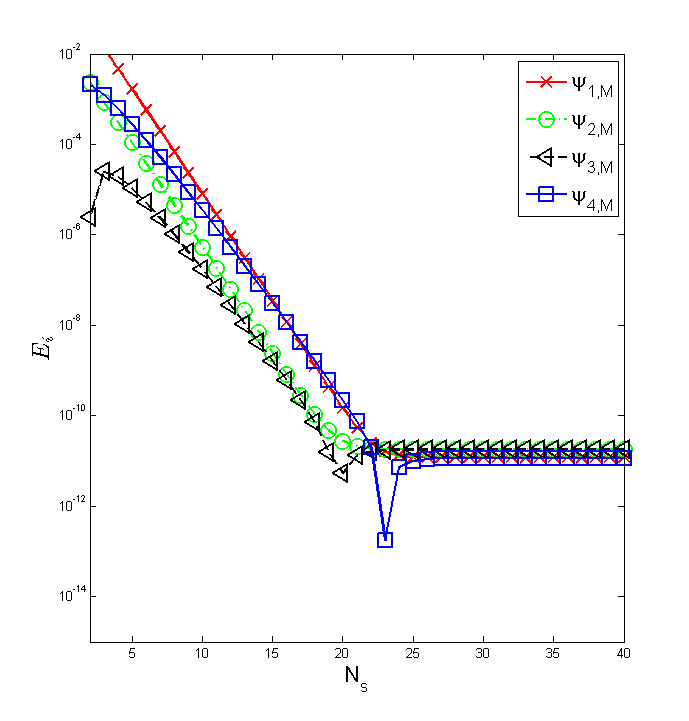
\includegraphics[width=2.5in]{err_gauss_to_matlab_exact.png}
		\caption{$E_i$ for quadrature test.}
		\label{fig:quad_err}
	\end{subfigure}
	\begin{subfigure}{0.45\textwidth}
		%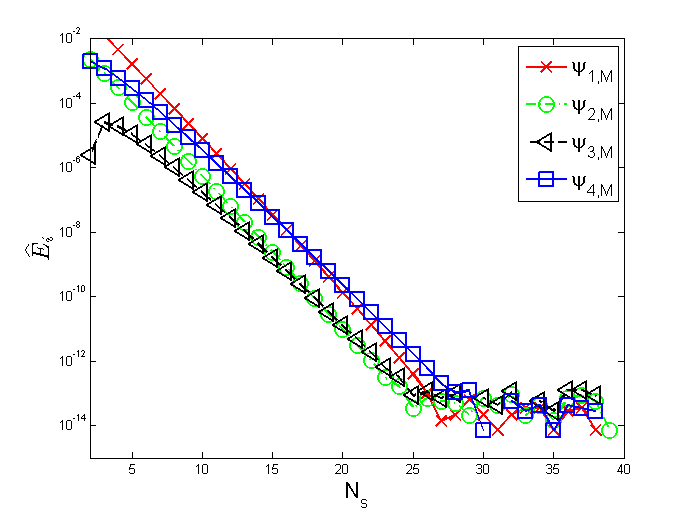
\includegraphics[width=2.5in,trim=0.5in  2.5in  1in 2.5in,clip=true]{err_gauss_to_highest_gauss.png}
		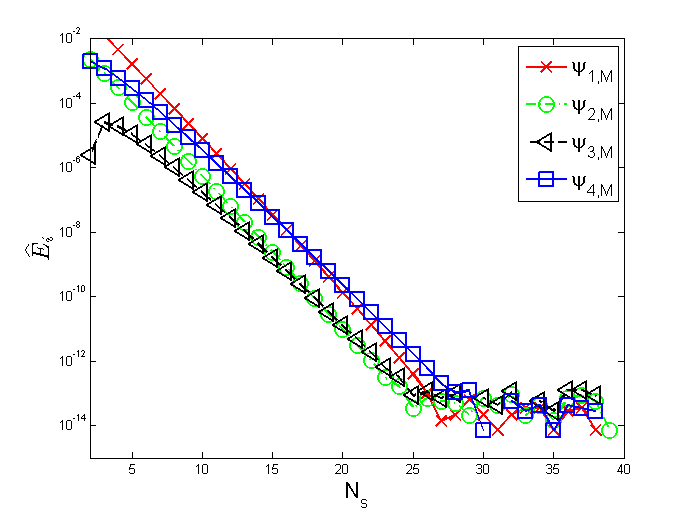
\includegraphics[width=2.5in]{err_gauss_to_highest_gauss.png}
		\caption{$\widehat{E}_i$ for quadrature test.}
		\label{fig:no_err}
	\end{subfigure}
\caption{Comparison of quadrature vs. exact integration errors.}
\label{fig:error_comparisons}
\end{center}
\end{figure}
As such, we prefer quadrature integration to evaluate cell integral quantities for the BCSZ scheme.
However, for a fixed number of Gauss points in $s$, we cannot apriori estimate the error in our quadrature approximation of bivariate polynomial integrals over the region with a curved boundary.
Gauss-Kronrod quadrature \cite{gk_quad} allows for an estimate of the quadrature approximation error of an integration.
In practice, we use the 7-point Gauss / 15-point Kronrod quadrature set in $s$ with a 2-point Gauss quadrature in $t$ to integrate all BCSZ quantities.
Using  sub-interval refinement, this quadrature integration strategy, and the decompositions shown in \fig{fig:bcsz_cases} allow for the computation of all BCSZ cell integral quantities to a tolerance less than our non-linear iteration tolerance.

\subsection{Non-linear Iteration}
To solve the four non-linear equations, we use Newton iteration with a finite difference formed Jacobian.
Additionally, we solve for ``well'' scaled values, using the first \BCSZH~ iterate ($\widetilde{\psi}_{UBLD}$) as a scaling vector.
As noted in \cite{csz_me,csz_don} solving for the non-linearity locally during each sweep precludes the use of Krylov methods in the scattering source iteration.

\section{Numerical Results}
\label{sec:results}
We now present computational results for a simple test problem, a $10~[cm] \times 10~[cm]$ void, with $S_4$ level symmetric angular quadrature,
 vacuum boundary conditions on the left, top, and right sides, incident angular flux of $1~[n/(cm^2-sec-ster)]$ in the direction of $\mu=0.868890300722,~\eta = 0.350021174582$ along the bottom edge, and vacuum conditions along the bottom edge for all other directions incident on the bottom face.
In \fig{fig:negatives} we compare the results of the UBLD, FLBLD, and BCSZ schemes on an orthogonal mesh of $64\times 64$ cells, plotting the cell average scalar fluxes on a logarithmic scale.
\begin{figure}[h]
	\begin{center}
		\begin{subfigure}{0.3\textwidth}
			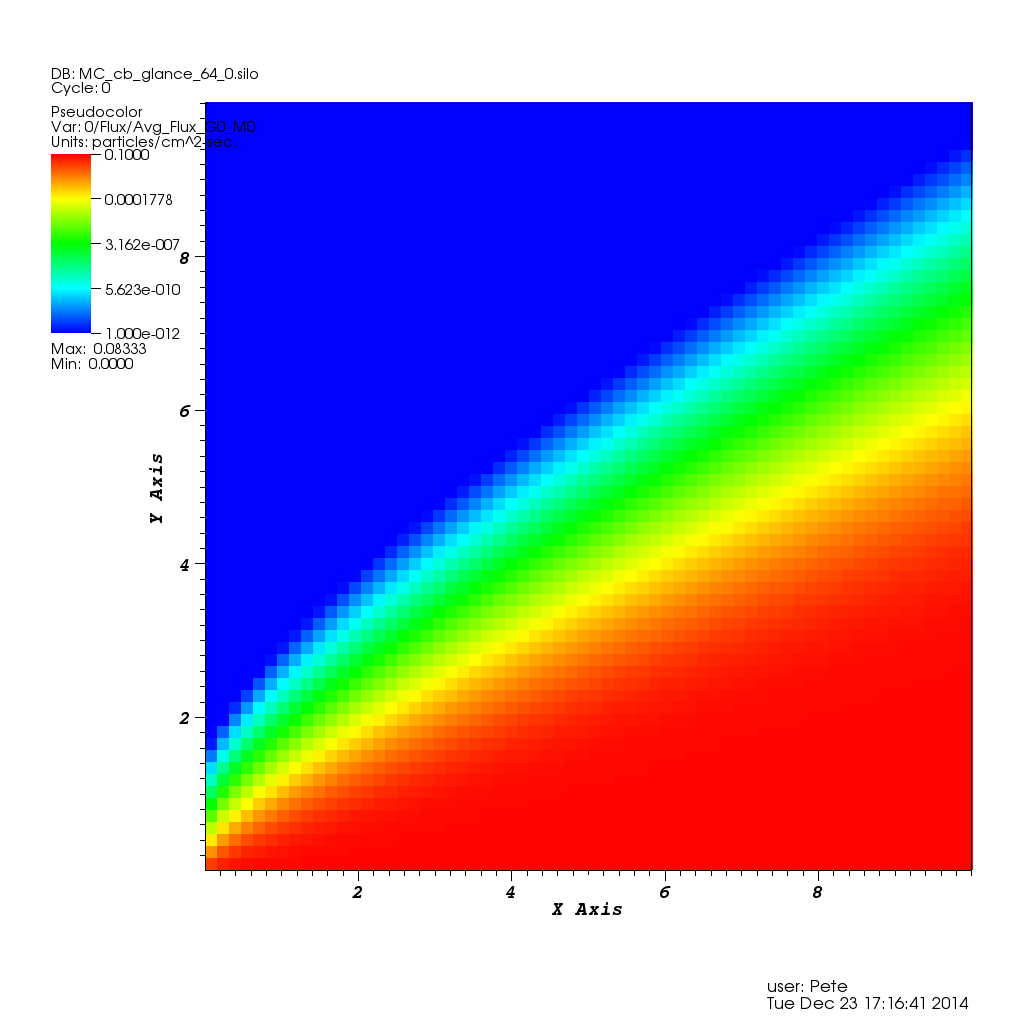
\includegraphics[width=2in]{cb_64.png}
			\caption{FLBLD solution}
			\label{fig:scb_64}		
		\end{subfigure}
		\begin{subfigure}{0.3\textwidth}
			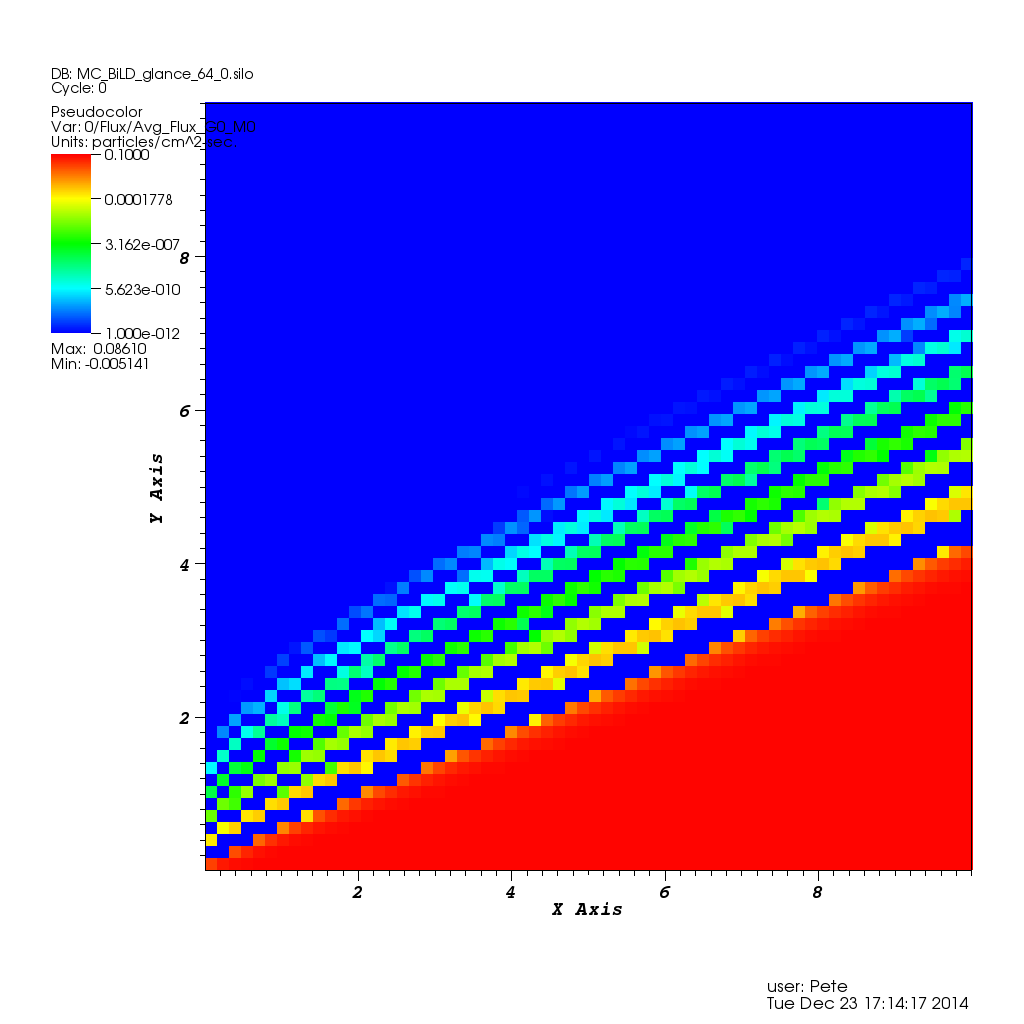
\includegraphics[width=2in]{bild_64.png}
			\caption{UBLD solution}
			\label{fig:bild_64}		
		\end{subfigure}
		\begin{subfigure}{0.3\textwidth}
			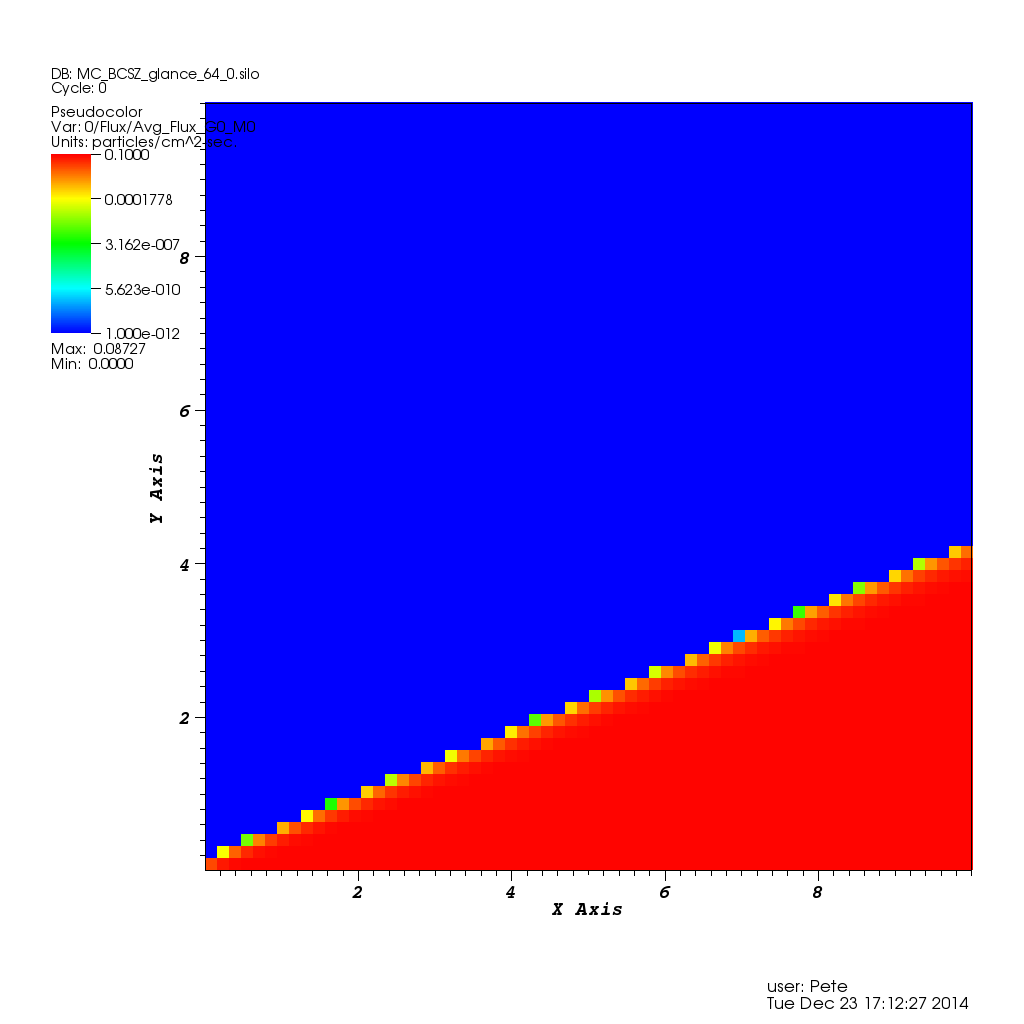
\includegraphics[width=2in]{bcsz_64.png}
			\caption{BCSZ solution}
			\label{fig:bcsz_64}		
		\end{subfigure}
	\end{center}
	\caption{$64\times 64$ mesh cell cell average scalar flux solutions}
	\label{fig:negatives}
\end{figure}
Plotting on a logarithmic scale accents the negativities and oscillations of the UBLD scheme.
Though undesirable, the negativities and oscillations of the UBLD dampen rapidly.  
The BCSZ and FLBLD solutions are both strictly non-negative.  
However, the FLBLD scheme has a significant amount of numerical diffusion, whereas the BCSZ scheme maintains a sharp boundary at the discontinuity.

In \fig{fig:unstructured} we show the BCSZ and UBLD cell average scalar flux solutions on a 25 cell $\times$ 25 cell mesh where each interior vertex has been randomly perturbed to create an unstructured mesh.
\begin{figure}[h]
	\begin{center}
	\begin{subfigure}{0.3\textwidth}
		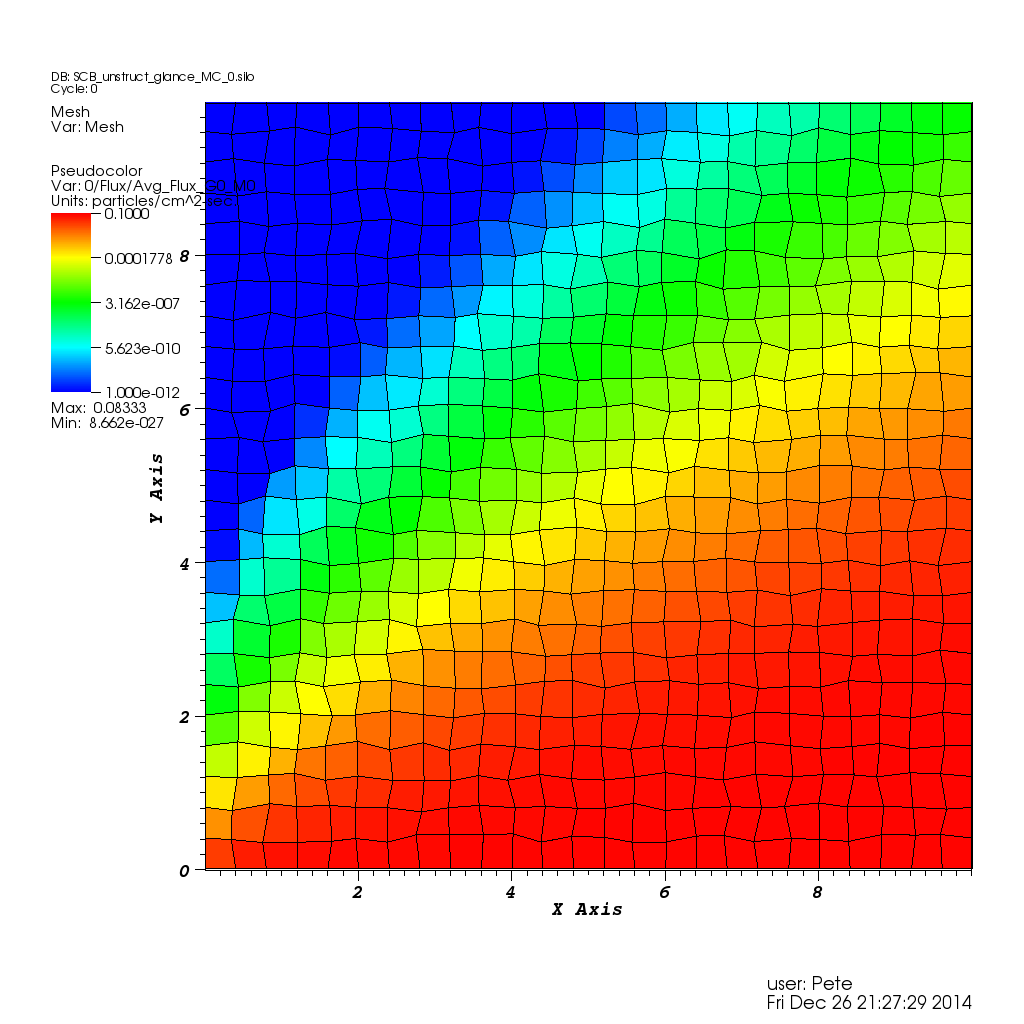
\includegraphics[width=2in]{scb_unstruct.png}
		\caption{FLBLD solution on unstructured grid.}		
		\label{fig:unstructured_scb}
	\end{subfigure}
	\begin{subfigure}{0.3\textwidth}
		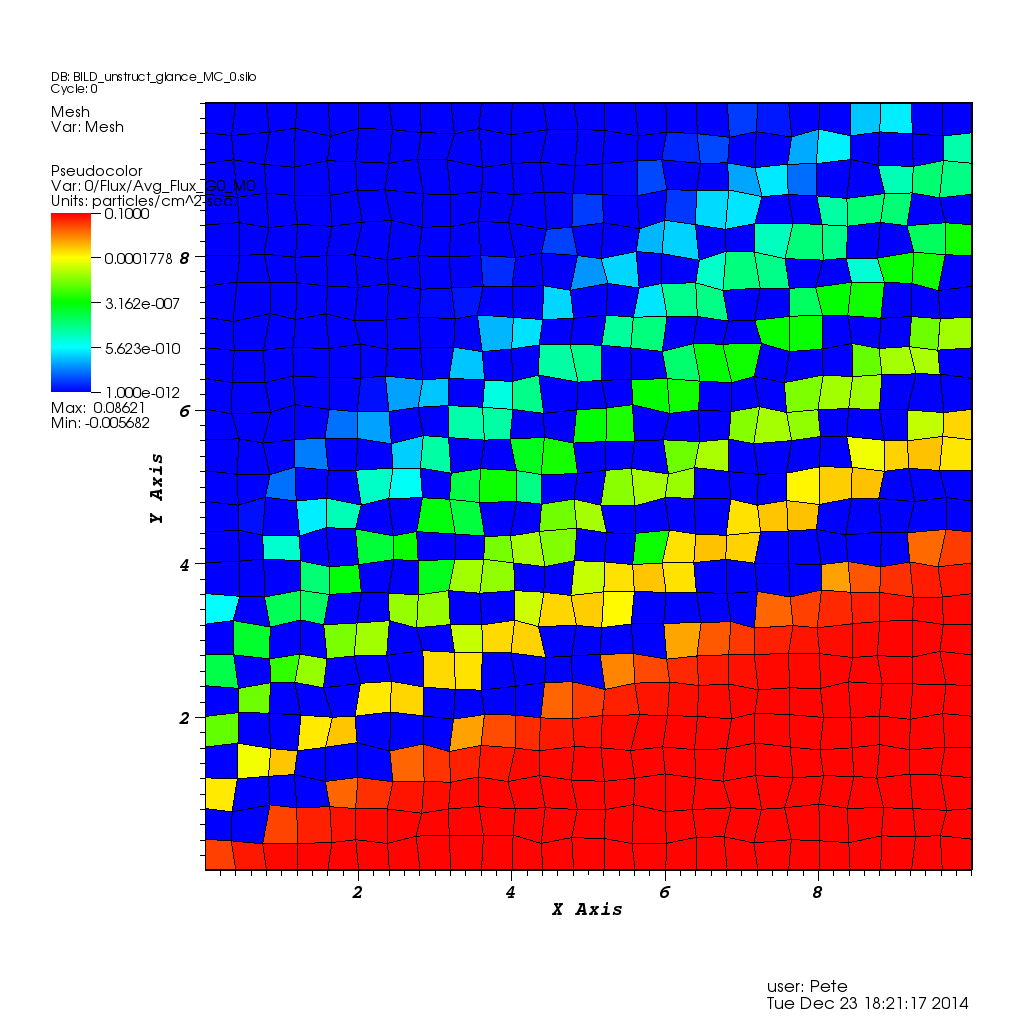
\includegraphics[width=2in]{bild_unstruct.png}
		\caption{UBLD solution on unstructured grid.}		
		\label{fig:unstructured_bild}
	\end{subfigure}
	\begin{subfigure}{0.3\textwidth}
		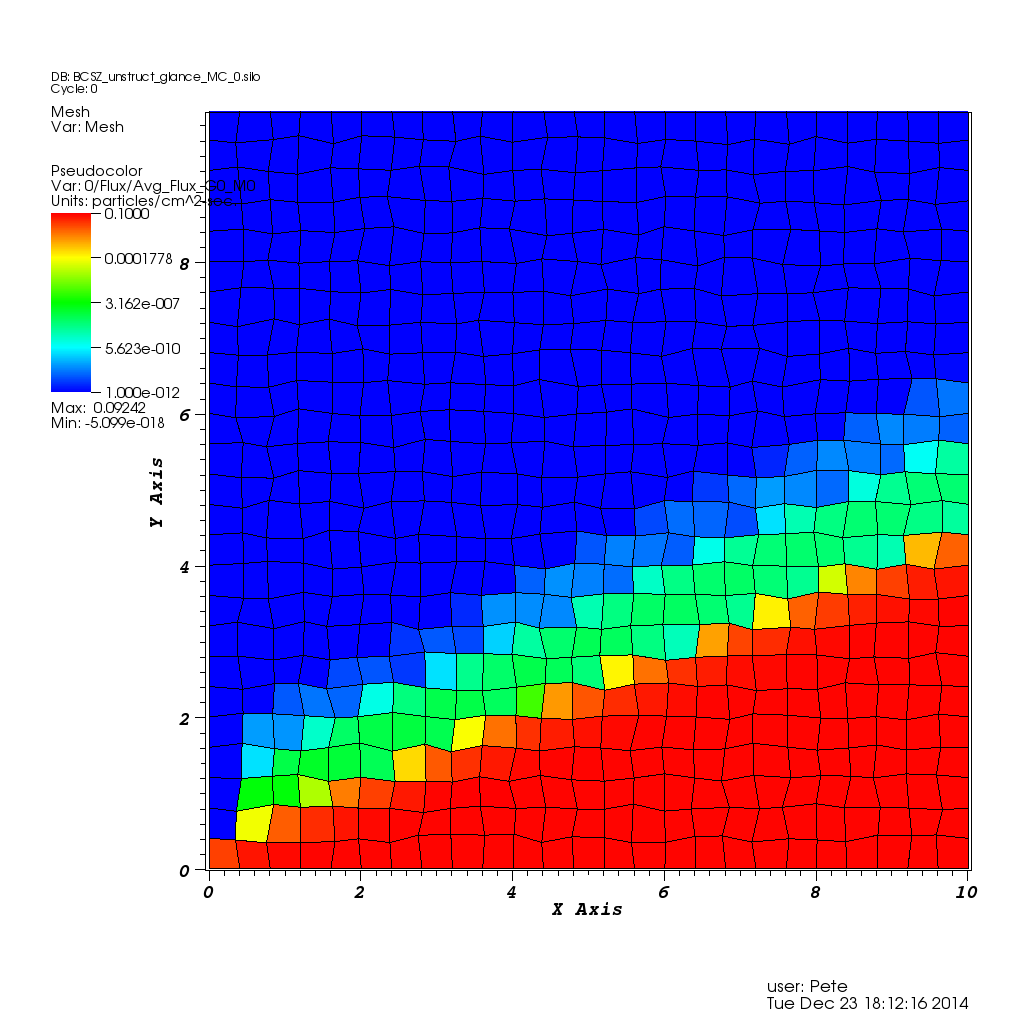
\includegraphics[width=2in]{bcsz_unstruct.png}
		\caption{BCSZ solution on unstructured grid.}
		\label{fig:unstructured_bcsz}
	\end{subfigure}		
	\caption{Glancing void solutions with $25\times 25$ mesh cells.}
	\label{fig:unstructured}
	\end{center}	
\end{figure}
Figure \ref{fig:unstructured} shows the BCSZ scheme is capable of being used for unstructured mesh problems.
Though the BCSZ solution exhibits numerical diffusion in \fig{fig:unstructured}, it is a result of the mesh, as both the FLBLD and UBLD schemes exhibit similar increases in numerical diffusion.  Again, the UBLD solution exhibits negativities and oscillations while the FLBLD and BCSZ solutions remain strictly non-negative.  In \fig{fig:unstructured}, the visible increase in BCSZ numerical diffusion is more an artifact of the logarithmic color scale, the averages in the cells with increased numerical diffusion are roughly a factor of $10^{-6}$ of the maximum angular flux average in any cell. 

Finally, in \fig{fig:convergence}, we plot $E_{\phi_A}$,
\benum
\label{eq:e_phi}
E_{\phi_A} = \sqrt{ \sum_{c=1}^{N_cells}{ \Delta x_c \Delta y_c (\widetilde{\phi}_A - \phi_{A,exact} )^2} } \pec
\eenum
an $L_2$ like norm of the average scalar flux in each cell for the UBLD, FLBLD, and BCSZ schemes on orthogonal meshes as a function of mesh size.  
In \eqt{eq:e_phi}, $\widetilde{\phi}_A$ is the computed cell average scalar flux for a particular scheme in cell $c$, $\Delta x_c$ and $\Delta y_c$ are the respective cell widths of cell $c$, and $\phi_{A,exact}$ is the analytic cell average scalar flux in cell $c$.
\begin{figure}[h]
\centering
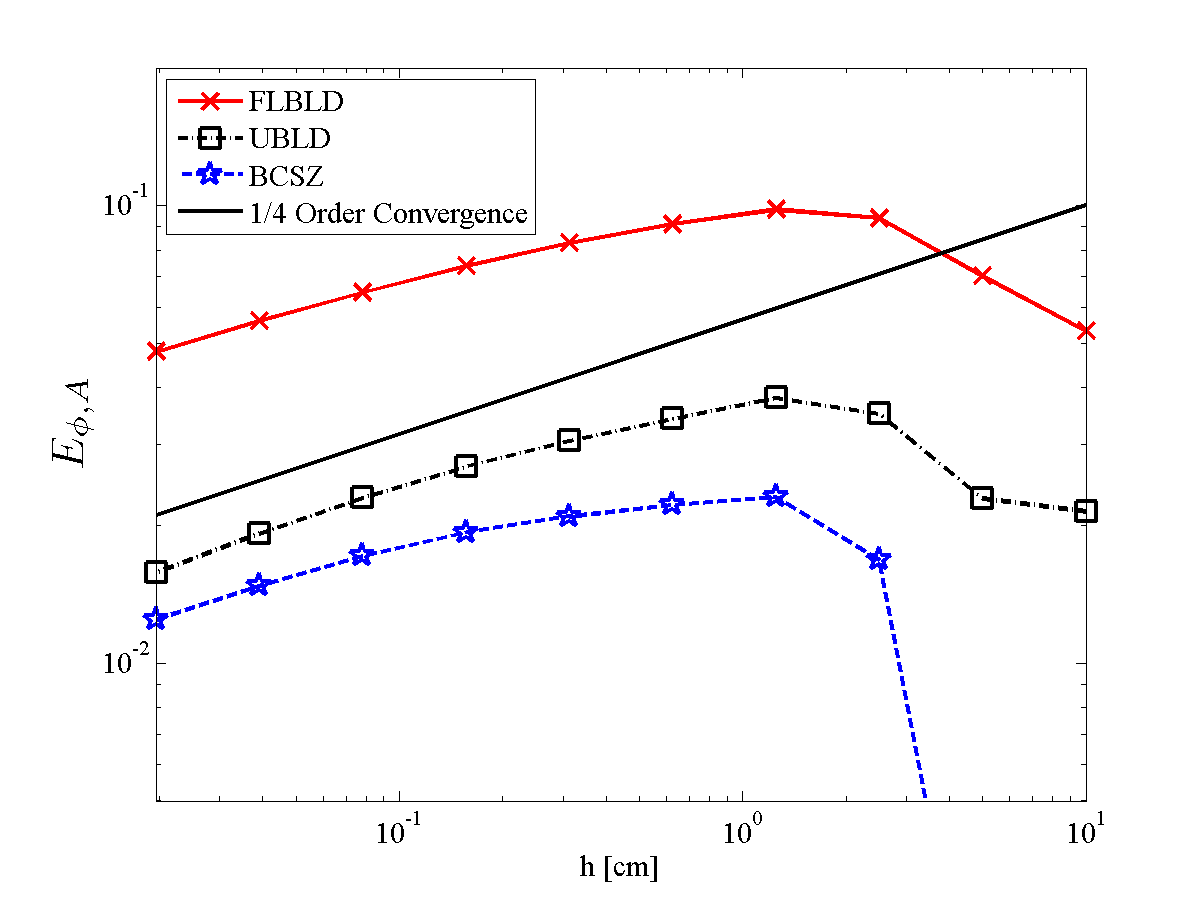
\includegraphics[width=4in]{glance_convergence}
\caption{Convergence of cell average scalar flux on orthogonal grids.}
\label{fig:convergence}
\end{figure}
From \fig{fig:convergence}, we see that BCSZ is more accurate than UBLD, while both UBLD and BCSZ are significantly more accurate than FLBD.
Also, we see that all methods reach the same asymptotic order of convergence, $h^{1/4}$.
All of the methods considered converge the error in the cell average angular flux at this low rate due to the discontinuity in the analytic solution.

\section{Conclusions}
\label{sec:conclusions}
The BCSZ scheme produces strictly non-negative solutions that are at least as accurate as UBLD solutions.
To date, the accuracy of the BCSZ scheme has only been measured against pure absorber/void test problems.  
We are currently awaiting the completion of a modified interior penalty  diffusion synthetic acceleration (MIP DSA) \cite{hackemack} implementation in the TAMU developed $S_N$ solver, PDT\cite{pdt}, to apply the BCSZ to more interesting neutron transport and radiative transfer problems.
We see numerous opportunities for future research going forward including:
\begin{enumerate}
\item developing appropriate timing problems to assess the computational cost of BCSZ relative to UBLD,
\item comparing the efficiency of our current/near term solution methodology (fixed point iteration with MIP DSA) to the solution methodology proposed by Bruss, et al. \cite{csz_don}, and
\item generalizing BCSZ to higher order, $Q_N$, trial spaces through the extension of adaptive quadrature integration (adaptive in both $s$ and $t$ to avoid finding where a $Q_N$ function is zero).
\end{enumerate}


%%%%%%%%%%%%%%%%%%%%%%%%%%%%%%%%%%%%%%%%%%%%%%%%%%%%%%%%% 

%\noindent
%The continuation of a paragraph after an equation is not indented

%\subsection{Subsection Title: First Character of Each Non-trivial Word is Uppercase}
%\subsubsection{Sub-subsection level and lower: only first character uppercase}
%
%Figures and tables should appear as closely as possible to where they are first cited, e.g. 
%Fig. \ref{fig:sample}, in the text.  Figures are numbered in Arabic numerals, with the caption centered below the figure, in boldface. 
%
%\begin{figure}[H]
  %\centering
  %%\includegraphics[width=3in]{figure.png}
  %\caption{Sample Figure. Color is permitted, but must be readable if printed.}
  %\label{fig:sample}
%\end{figure}
%
%When importing figures or any graphical image please verify two things:
%\begin{enumerate}
%\item Any number, text or symbol is no smaller than 10-point after reduction to the actual window in your paper;
%\item That it can be translated into PDF.
%\end{enumerate}
%
%Tables, like Table \ref{tab:sample}, are numbered in Roman numerals, with the caption centered above the table, in \textbf{boldface}.  
%Double-space before and after the table.
%
%\begin{table}
  %\centering
  %\caption{Sample table: accuracy of nodal and characteristic methods}
  %\begin{tabular}{lcccc}
    %\toprule
    %Mesh & 8 x 8 & 16 x 16 & 32 x 32 & 64 x 64 \\
    %\midrule
    %Nodal & \num{1.000e-1} & \num{2.500e-2} & \num{6.250e-3} & \num{1.563e-3} \\
    %Characteristic & \num{1.000e-1} & \num{2.500e-2} & \num{6.250e-3} & \num{1.563e-3} \\
    %\bottomrule
  %\end{tabular}
  %\label{tab:sample}
%\end{table}


%%%%%%%%%%%%%%%%%%%%%%%%%%%%%%%%%%%%%%%%%%%%%%%%%%%%%%%%%%%%%%%%%%%%%
\section{Acknowledgments}

Portions of this work were funded by the Department of Energy CSGF program, administered by the Krell Institute, under grant DE-FG02-97ER25308.

%%%%%%%%%%%%%%%%%%%%%%%%%%%%%%%%%%%%%%%%%%%%%%%%%%%%%%%%%%%%%%%%%%%%%
\setlength{\baselineskip}{12pt}

\bibliographystyle{mc2015}
\bibliography{references}

%%%%%%%%%%%%%%%%%%%%%%%%%%%%%%%%%%%%%%%%%%%%%%%%%%%%%%%%%%%%%%%%%%%%%
%\appendix
%\section{}
%
%If necessary, include Appendices numbered in upper case alphabetical order.
%
%In order to ensure a uniform, professional look to the proceedings, please
%\emph{\textbf{do not modify}} the format of this template without checking with
%the organizers first.

\end{document}
